
\section{Qualitative Analysis}
\section{Approach}

For $M$ modalities, we define a distance based loss function which is a generalization of well-known similarity-based metric learning and manifold alignment methods such as triplet loss~\cite{Carvalho-cooking-triplet,triplet_loss_2021_CVPR}, quadruplet loss~\cite{chen2017beyond}, and is similar to contrastive loss under some settings.
We sample two data points from each modality, one positive point and one negative point. 
For each set of positive data points (referring to an instance of an object with all of its modalities), we choose a set of negative data points either based on object class name, or by semantic negative sampling~\cite{Pillai_Matuszek_2018}. We now have two data points; we consider the first one as positive, and the second one as negative. However, the anchor won't be another data point as it is in the triplet loss terminology. Instead we choose one domain as an anchor. 

\begin{itemize}
    % \item data point: a row in the csv/tsv file.
    \item Positive: a set of embeddings of the one data point (RGB image of an apple, corresponding depth image, text description, and speech description of the same apple)
    \item Negative: a set of embeddings of the another data point of a different object (RGB image of a book, corresponding depth image, text description, and speech description of the same book)
    \item Anchor: A fixed modality to act as anchor in the case of simple MMA loss, where we don't minimize the distance between the pair of embeddings from all modalities of the same data point, and we don't maximize the distance between positive an negative datapoints of the same modality.
\end{itemize}

The objective is then to (I) minimize the distance between each pair of positive points from heterogeneous modalities which results in $(M-1)!$ terms, (II) maximize the distance between each pair of positive and negative points from heterogeneous modalities which contains $(M-1)!$ terms again, and (III) maximize the distance between each pair of positive and negative points from the homogeneous modalities which contains $M$ terms. Altogether, our proposed loss function contains $M+2(M-1)!$ terms.
\Cref{eq:objective} shows the objective function we defined above with changing maximization to minimization by changing the sign.

% \begin{equation}\label{eq:objective-detailed}
%     \min \sum_{i=1}^{M-1} \sum_{j=i+1}^{M} ||x_{i}^{+} - x_{j}^{+}|| - \sum_{i=1}^{M-1} \sum_{j=i+1}^{N} ||x_{i}^{+} - x_{j}^{-}|| - 
%     \sum_{i=1}^{M} ||x_{i}^{+} - x_{i}^{-}||
% \end{equation}


% \begin{equation}\label{eq:objective}
% \begin{split}
%     \mathcal{L}  &= \sum_{i=1}^{M-1} \sum_{j=i+1}^{M} ||f_i(x_{i}^{+}) - f_j(x_{j}^{+})|| \\
%     & - ||f_i(x_{i}^{+}) - f_j(x_{j}^{-})||
%     - ||f_i(x_{i}^{-}) - f_j(x_{j}^{+})|| \\
%     & - \sum_{i=1}^{M} ||f_i(x_{i}^{+}) - f_i(x_{i}^{-}) ||
% \end{split}
% \end{equation}
% where $f_i(.)$ and $f_j(.)$ represent functions that map input data to the shared latent space using a deep neural network.


% d(,) notation instead of || - ||
% \begin{equation}\label{eq:objective}
% \begin{split}
%     \mathcal{L}  &= \sum_{i=1}^{M-1} \sum_{j=i+1}^{M} d(z_{i}^{+}, z_{j}^{+}) 
%      - d(z_{i}^{+}, z_{j}^{-}) \\ 
%     & - d(z_{i}^{-}, z_{j}^{+}) - \sum_{i=1}^{M} d(z_{i}^{+}, z_{i}^{-})
% \end{split}
% \end{equation}

\begin{equation}\label{eq:objective}
\begin{split}
    \mathcal{L}  &= \sum_{i=1}^{M-1} \sum_{j=i+1}^{M} ||z_{i}^{+} - z_{j}^{+}|| 
     - ||z_{i}^{+} - z_{j}^{-}|| - ||z_{i}^{-} - z_{j}^{+}|| \\ 
    &  - \sum_{i=1}^{M} ||z_{i}^{+} - z_{i}^{-} ||
\end{split}
\end{equation}
where the subscripts $i$ and $j$ represent modalities, and $z$ is the embedding we get by applying a mapping function $f$ which in our case is a neural network on our input data. In other words $z_m = f_m(x_m)$ where each modality $m$ has a specific model $f_m$ that is different from the models for other modalities and these models do not share their weights. 
To measure the distance, we use cosine distance.
In order to use cosine \textit{distance}, we have to subtract the cosine of the \textit{angle} between two embeddings (which represents similarity) from 1: $1 - \cos(e_1, e_2)$.

\todokdinline{I can add another term for minimizing the distance between similar pairs (anchor and positive) from the same domain. This would look like the equation below. However, it breaks the nice procedure of sampling two data points per modality}
\todo{Edward wonders if $f_i(x)$ should instead produce $\mu_x$ and $\Sigma_x$, to capture uncertainty of embedding location, when working with so many modalities? (e.g., not all modalities share the same ambiguities)}
\todo{Does Edward mean the actual network produces $\Sigma_x$, e.g., something like a VAE? How would uncertainty be applied to the inference problem?}
$+ \sum_{i=1}^{M} ||f_i(x_i^{a}) - f_i(x_i^{+})||$


If $M=2$ which means the number of modalities is 2, then our objective function reduces to the quadruplet loss method~\cite{chen2017beyond} if we ignore the third term, and negative samples for each modality do not belong to the same class.
If $M=2$ and we ignore the last two terms in the objective function, it results in the triplet loss method. 
If $M=1$, only the last term remains in the loss function which is exactly the pairwise distance-based loss function.


We demonstrate performance using three different distance-based loss functions.
\todokdinline{Either remove it or experiment with all versions of MMA (12 terms, 9 terms, and explicit anchor maximization}

\subsection{Simple MMA}
\label{sub:simple-mma}
Our first proposed loss function is a modification of the triplet loss function idea, and can be derived from \cref{eq:objective} by fixing one modality as anchor, and ignoring the last two terms in \cref{eq:objective}.

% For each data point (referring to an instance of an object with all of its modalities), we choose a negative data point either based on object class name, or by semantic negative sampling~\cite{Pillai_Matuszek_2018}. We now have two data points; we consider the first one as positive, and the second one as negative. However, the anchor won't be another data point as it is in the triplet loss terminology. Instead we choose one domain as an anchor. 

% \begin{itemize}
%     % \item data point: a row in the csv/tsv file.
%     \item Positive: a set of embeddings of the one data point (RGB image of an apple, depth image of an apple, language description of an apple)
%     \item Negative: a set of embeddings of the another data point of a different object (RGB image of a book, depth image of a book, language description of a book)
%     \item Anchor: A fixed modality to act as anchor in the case of simple MMA loss, where we don't minimize the distance between the pair of embeddings from all modalities of the same data point, and we don't maximize the distance between positive an negative datapoints of the same modality.
% \end{itemize}

Since the downstream task in the grounded language learning domain is to predict/retrieve a desired object among multiple objects given a natural language description, it makes sense to train the model using language as an anchor, and in fact anchoring learning around language outperforms anchoring on RGB.

\Cref{eq:objective-simple-mma} shows the mathematical formulation of the proposed loss function which can be generalized to arbitrary number of modalities.

% \begin{equation}
% \label{eq:objective-simple-mma}
% \begin{split}
%     \mathcal{L}  &= \sum_{m=1}^{M-1} || f_a(x_{a}^{+}) - f_m(x_{m}^{+}) || - \\ 
%     & || f_a(x_{a}^{+}) -f_m(x_{m}^{-}) || 
%     \\
%     &= \sum_{m=1}^{M-1} 1 - \cos(f_a(x_{a}^{+}), f_m(x_{m}^{+})) \\ & - (1 - \cos(f_a(x_{a}^{+}) ,f_m(x_{m}^{-}))) \\
%     &= \sum_{m=1}^{M-1} \cos(f_a(x_{a}^{+}) ,f_m(x_{m}^{-})) \\ 
%     & - \cos(f_a(x_{a}^{+}), f_m(x_{m}^{+}))
% \end{split}
% \end{equation}

\begin{equation}
\label{eq:objective-simple-mma}
\begin{split}
    \mathcal{L}  &= \sum_{m=1}^{M-1} || z_{a}^{+} - z_{m}^{+} || - || z_{a}^{+} - z_{m}^{-} || \\
    &= \sum_{m=1}^{M-1} 1 - \cos(z_{a}^{+}, z_{m}^{+}) - (1 - \cos(z_{a}^{+}, z_{m}^{-})) \\
    &= \sum_{m=1}^{M-1} \cos(z_{a}^{+} ,z_{m}^{-}) - \cos(z_{a}^{+}, z_{m}^{+})
\end{split}
\end{equation}

where subscript $a$ represents \textit{anchor} modality, $M$ is the number of modalities, superscript $+$ represents the positive objects, and superscript $-$ represents the negative objects.

An illustration of this loss function is provided in \cref{fig:simple-mma-loss}.

\begin{figure}[tb]
\centering
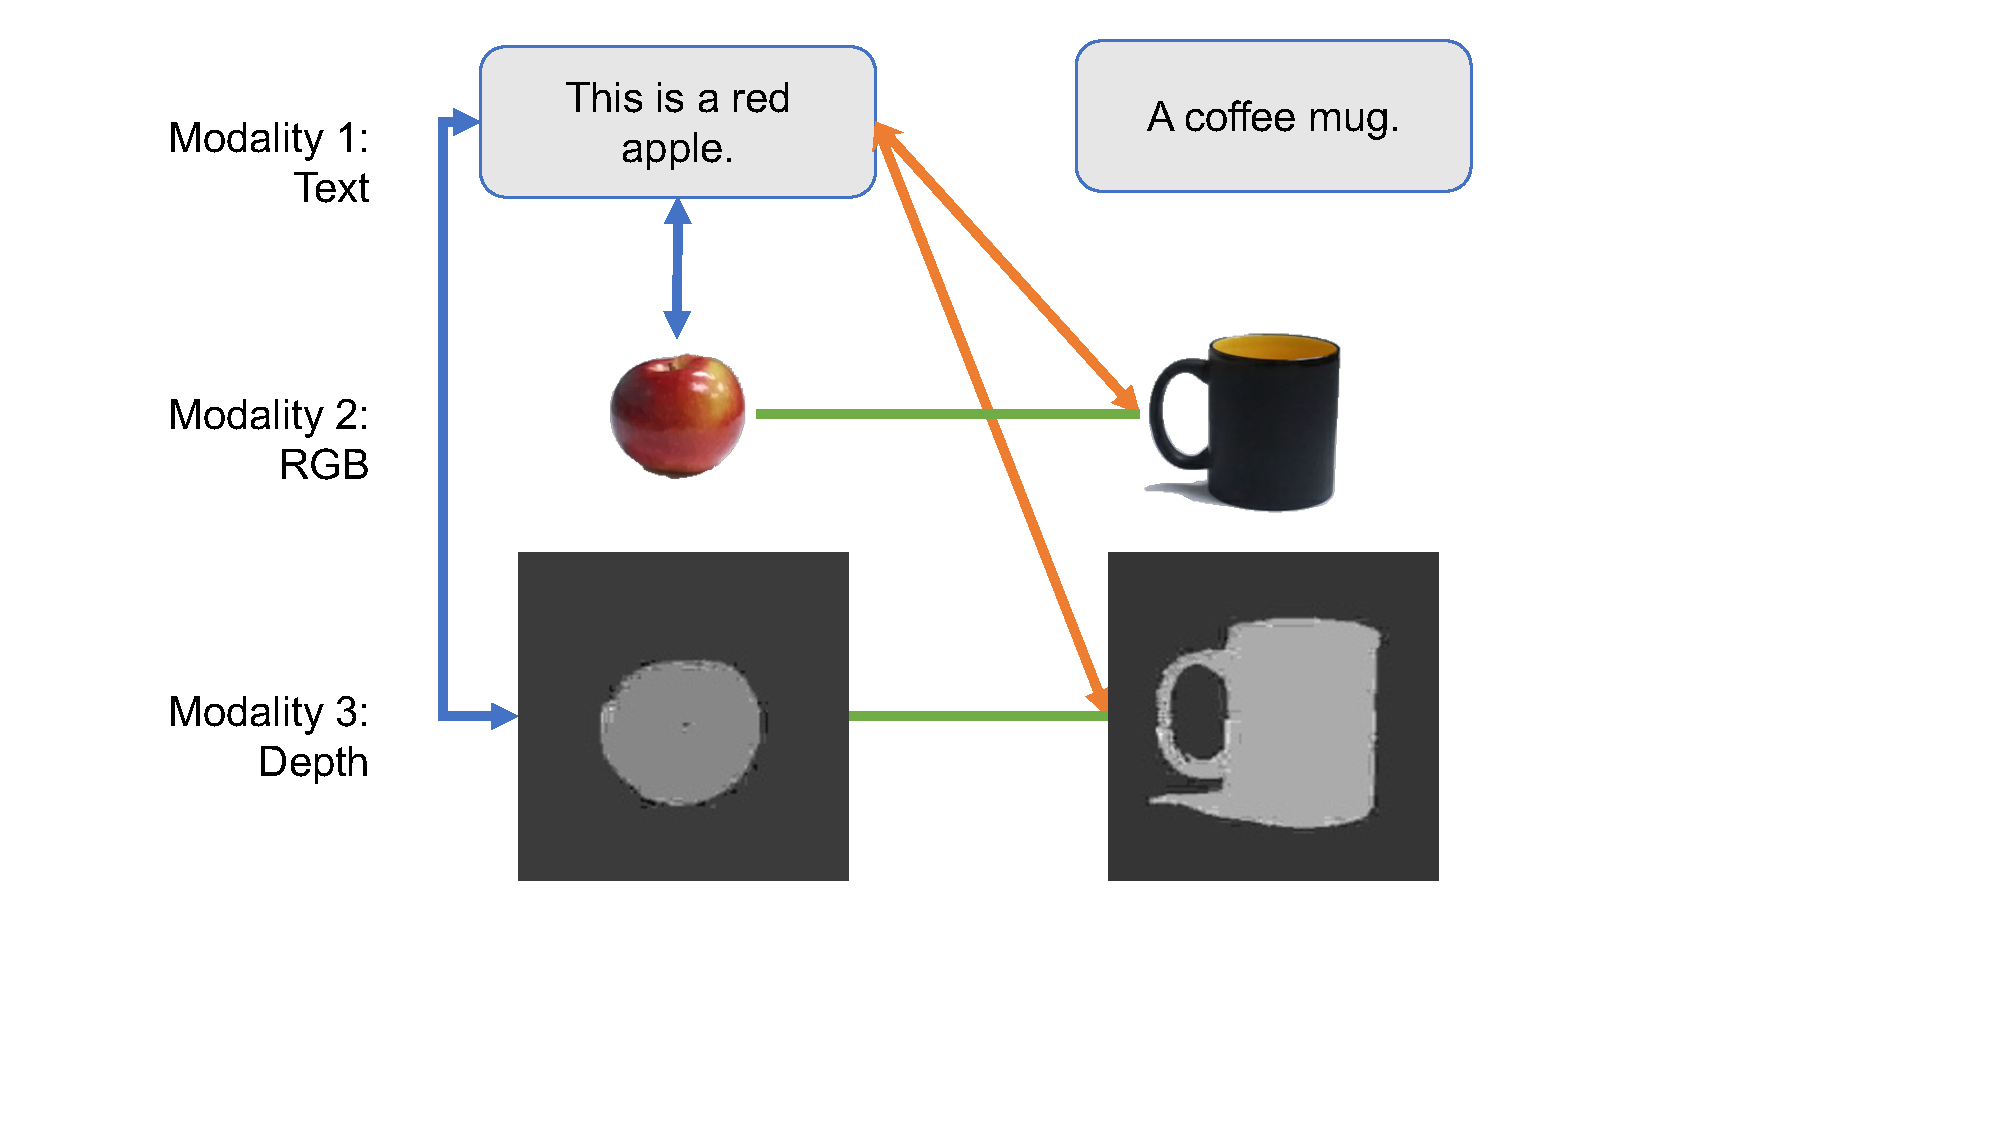
\includegraphics[width=\columnwidth]{Figures/simple-MMA.pdf}
\caption{A high-level prototype of the distances used in the simple MMA loss with 3 modalities. Orange arrows indicate maximizing the distance, blue arrows indicate minimizing the distance, and green lines show the margin. Depth images are brightened to be visible. \todo[inline]{We need to show speech as the 4th modality as well.}}
\label{fig:simple-mma-loss}
\end{figure}

This version of MMA loss function can be seen as a contrastive loss usually used in the domain of self-supervised learning~\cite{chen2020simple}. However, our proposed loss function has two advantages over the traditional contrastive loss expressed in \cref{eq:contrastive-loss}. The first advantage is that our loss function do not loop over multiple positives and negatives in a large batch. Instead we sample only two objects (positive and negative) each of which have $M$ modalities which gives us $2M$ datapoints (or embeddings). Hence, our model can be trained using smaller batch sizes and reduces the number of negative samples we need. The second advantage is that this loss function can be used in a multimodal setting with an arbitrary number of modalities, and is not limited to a single data type (e.g. RGB images) which is the most common usage of contrastive loss~\cite{chen2020simple, NEURIPS2020_supervised_contrastive}.


Therefore, our proposed loss function would modify \cref{eq:contrastive-loss} to the loss function formulated in \cref{eq:simple-MMA-contrastive}. Our formulation is a generalized version of the contrastive loss where $M$ is the number of modalities (e.g. RGB image, depth image, speech, text), but it can be the ``augmented views'' instead of different modalities.

% \begin{equation}\label{eq:simple-MMA-contrastive}
%     -\sum_{m=1}^{M-1} \log \frac{\exp (sim(f_a(x_a^+) , f_m(x_{m}^{+})/ \tau) )}{ \exp (sim(f_a(x_a^+) , f_m(x_{m}^{+}) / \tau)) + \exp (sim(f_a(x_a^+), f_m(x_{m}^{-}) / \tau))}
% \end{equation}

\begin{equation}\label{eq:simple-MMA-contrastive}
    -\sum_{m=1}^{M-1} \log \frac{\exp (sim(z_a^+ , z_{m}^{+})/ \tau) }{ \exp (sim(z_a^+ , z_{m}^{+}) / \tau) + \exp (sim(z_a^+, z_{m}^{-}) / \tau)}
\end{equation}
where $z = f(x)$.

% \todokdinline{I should run the traditional contrastive loss to see if my method works better to make this claim.}



% \subsubsection{All in loss with 12 terms}
% \subsubsection{subset of All in loss with 9 terms}

\section{Data}

\begin{figure*}[tbh]
\centering
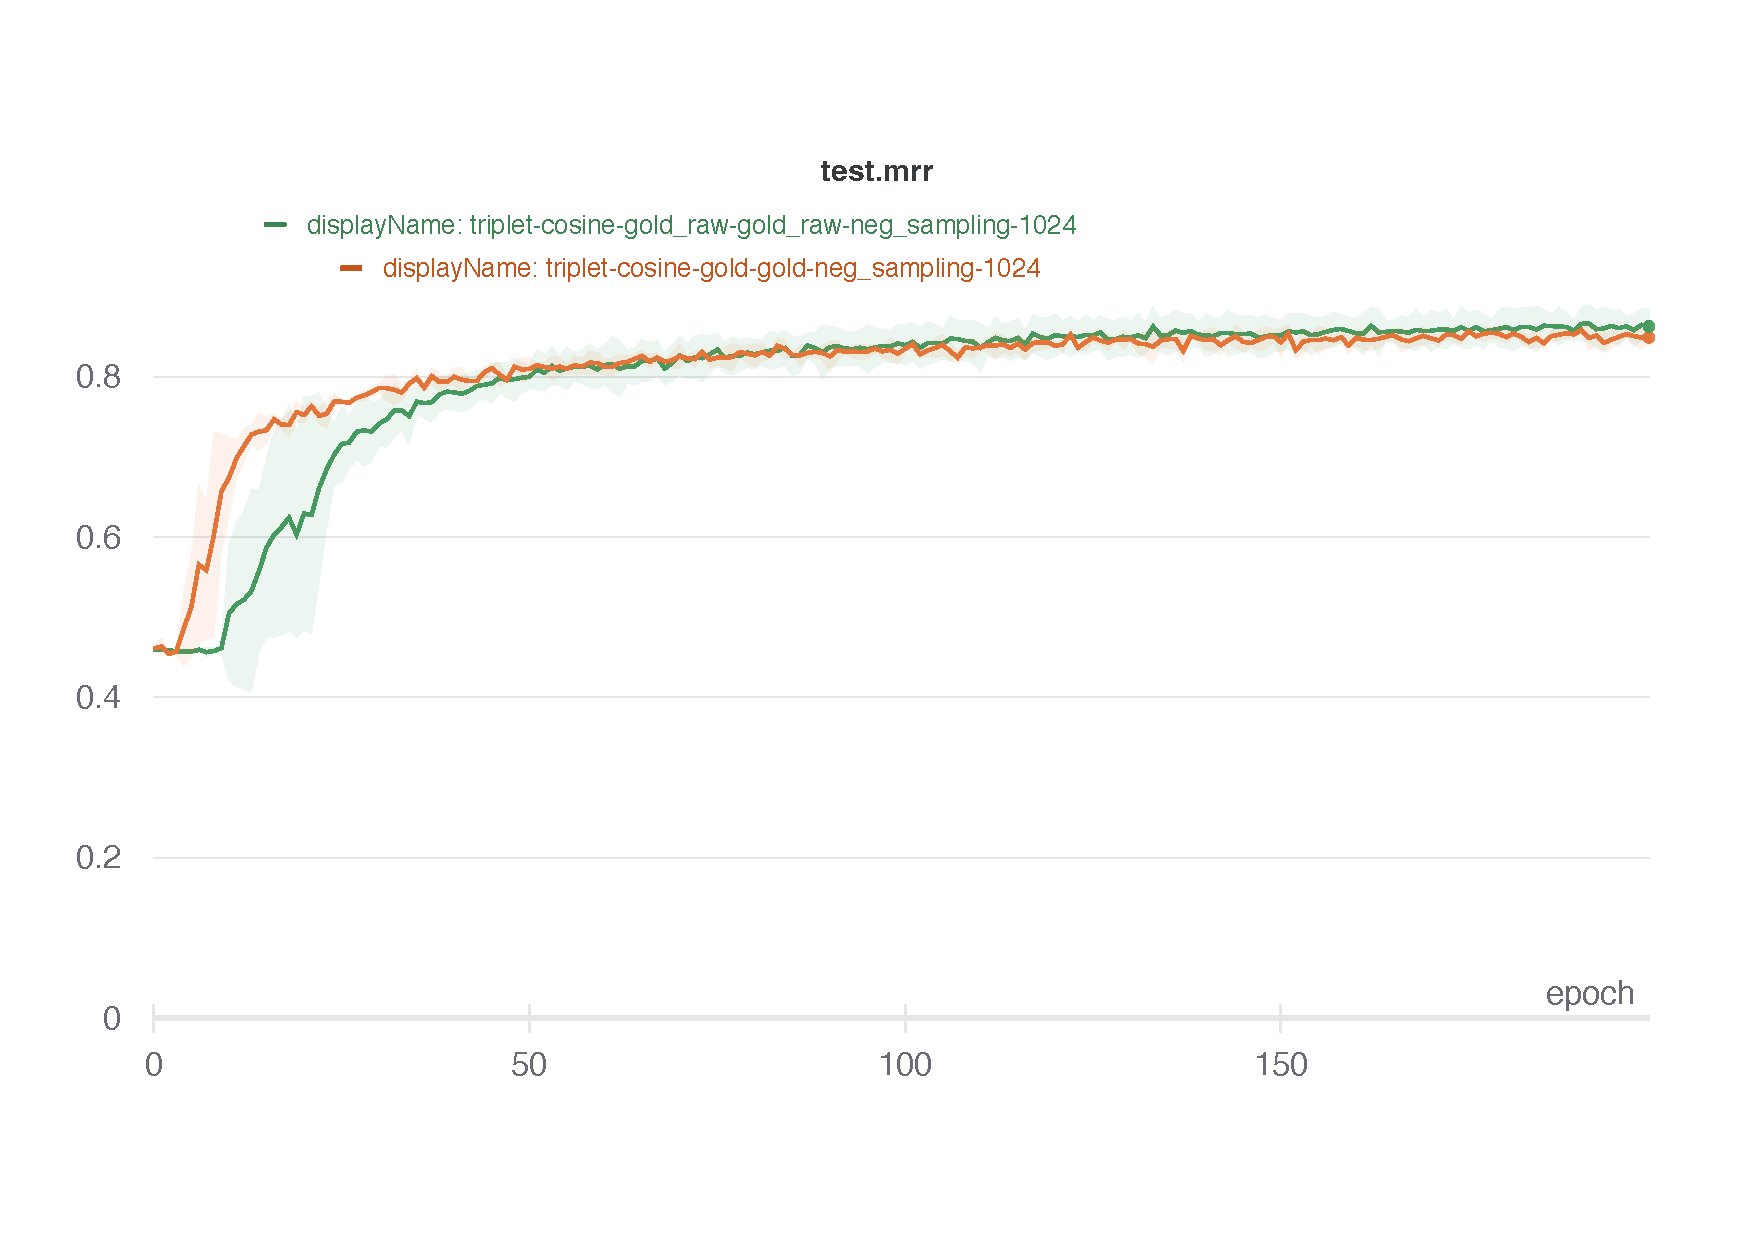
\includegraphics[width=2.0\columnwidth]{Figures/raw-mask-test-mrr.pdf}
\caption{Mean Reciprocal Rank (MRR) on different versions of GoLD dataset~\cite{GoLD_UMBC}. The raw version is depicted in green and masked version is depicted in orange averaged over 3 different random seeds. Higher is better.}
\label{fig:mask-vs-raw}
\end{figure*}

\section{Experiments}

\section{Results}

\begin{figure*}[tbh]
\centering
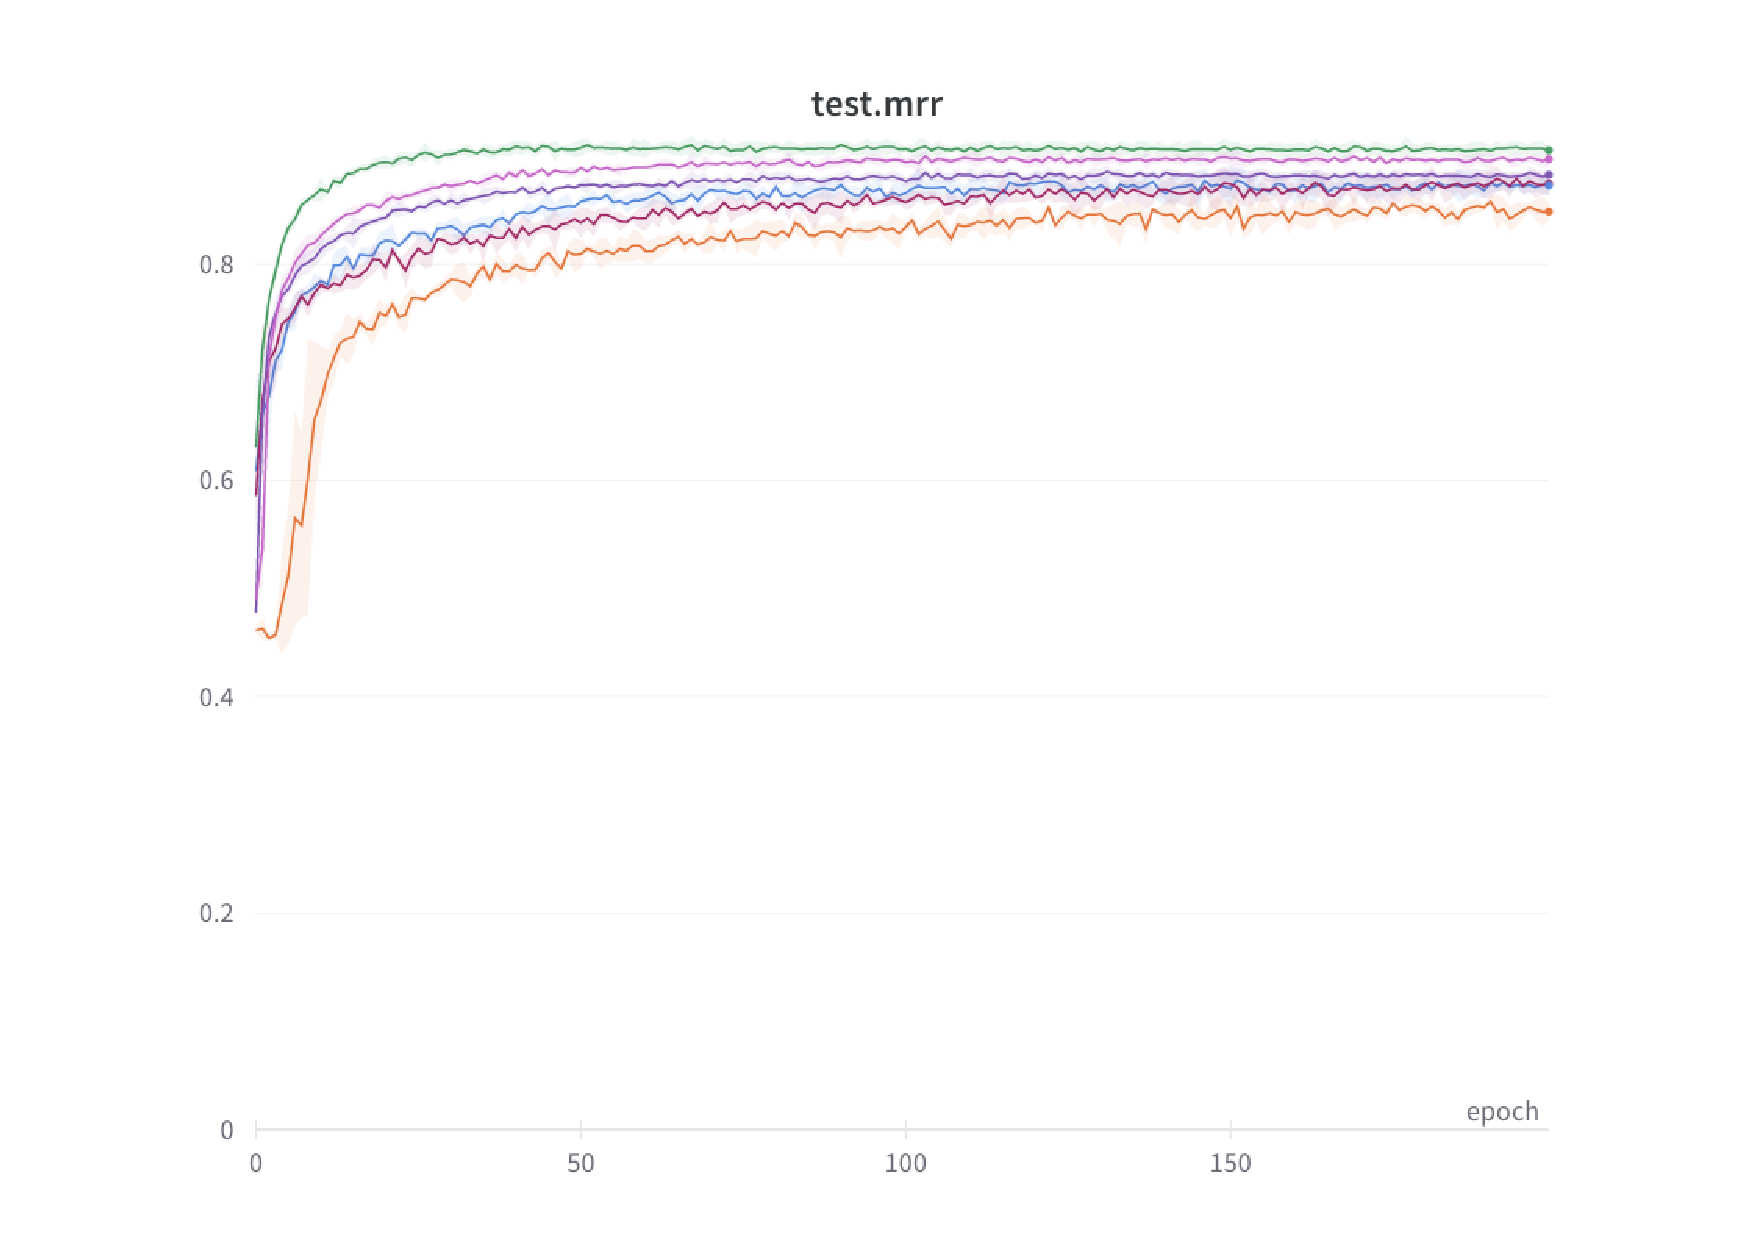
\includegraphics[width=2.1\columnwidth]{Figures/test.mrr.pdf}
\caption{Mean Reciprocal Rank (MRR) of our proposed method against triplet loss method averaged over 3 different random seeds for a downstream task of object detection. The higher is better. Green is Supervised Contrastive Learning~\cite{NEURIPS2020_supervised_contrastive}, Pink represents our proposed simple MMA loss function without semantic negative sampling w/ SGD w/ adjusting learning rate, Purple is out method with semantic negative sampling, Blue is our method w/ semantic negative sampling w/ Adam and w/o adjusting learning rate, Red is vanilla contrastive loss with cosine, and orange represent the triplet loss. function~\cite{triplet_loss_2021_CVPR}.
}

\label{fig:simple-MMA-mrr}
\end{figure*}

\section{Setup}

% \section{Lit Search}
\subsection{Multimodal Machine Learning: A Survey and Taxonomy}

\begin{itemize}
\item \href{https://ieeexplore.ieee.org/document/8269806}{url}
\end{itemize}

\citet{baltrusaitisMultimodalMachineLearning2019} proposes a new taxonomy of multimodal machine learning by introducing five technical challenges in addition to typical early and late fusion categorization. This taxonomy includes the following categories.
\begin{enumerate}
\item \textit{Representation}: represent and summarize multimodal data in a way that exploits the complementarity and redundancy of multiple modalities.
\begin{enumerate}
\item joint: combine the unimodal signals into the same representation space.
\item coordinated: process unimodal signals separately, but enforce certain similarity or structure constraints on them to bring them to a coordinated space.
\end{enumerate}
\item \textit{Translation}: map data from one modality to another.
\begin{enumerate}
\item example-based
\item generative
\end{enumerate}
\item \textit{Alignment}: identify the direct relations between (sub)elements from two or more different modalities.
\begin{enumerate}
\item explicit
\item implicit
\end{enumerate}
\item \textit{Fusion}: join information from two or more modalities to perform a prediction.
\begin{enumerate}
\item model-agnostic
\item model-based
\end{enumerate}
\item \textit{Co-learning}: transfer knowledge between modalities, their representation, and their predictive models
\begin{enumerate}
\item parallel data
\item non-parallel data
\item hybrid data
\end{enumerate}
\end{enumerate}

The authors mention that while joint representations have been used in situations to construct representations of more than two modalities, coordinated spaces have, so far, been mostly limited to two. This means that our research is novel and we can extend similarity measures to more than two modalities.

\subsection{Self-Supervised MultiModal Versatile Networks}

\begin{itemize}
\item \href{https://proceedings.neurips.cc/paper/2020/file/0060ef47b12160b9198302ebdb144dcf-Paper.pdf?utm\_campaign=NLP\%20News\&utm\_medium=email\&utm\_source=Revue\%20newsletter}{url}
\end{itemize}


This work uses self-supervised contrastive learning to learn and combine representations from three modalities of visual, audio, and language. They learn a \textit{multimodal versatile network} that has the following four properties:
\begin{enumerate}
\item Ability to take any of the modalities as input
\item Respecting the specificity of modalities: audio and visual modalities are fine-grained while language modality is coarse-grained.
\item Comparability of different modalities using \textbf{dot product} even if not seen together during training 
\item Efficiently applicable to visual data either in the form of dynamic videos or static images
\end{enumerate}


The authors consider the following three different configurations of the modality spaces which they call \textit{modality embedding graphs}.
\begin{enumerate}
\item Shared: all modalities map to the same space. This respects property 3 but violates property 2.
\item Disjoint: visual-audio and visual-text spaces. This respects property 2 but violates property 3.
\item Fine and coarse: audio and visual domains are map to the same space since they are fine-grained. These embeddings are then mapped to a lower dimensional space where text is also mapped. This respects both properties 2 and 3.
\end{enumerate}

The loss function they define consists of two terms. The first term is to train the fine-grained space of visual and audio embeddings by minimizing the distance between the similar pair (positives) from the same location of a video, and maximizing the distance between negative pairs (negatives) sampled from different videos. The second term is to train the coarse-grained space which consists of visual and text embeddings. Note that they don't consider audio embeddings in this space since they don't want to learn automatic speech recognition (ASR). Text and visual domains are not aligned as well as audio and visual domains (e.g. sound of playing piano versus the text that only says playing piano for a video of playing piano). To cure this, they consider a set of positive pairs instead of a single pair.
If a modality is missed, the corresponding term is dropped from the loss function.

\subsection{Separating Self-Expression and Visual Content in Hashtag Supervision}

\begin{itemize}
\item \href{https://openaccess.thecvf.com/content\_cvpr\_2018/papers/Veit\_Separating\_Self-Expression\_and\_CVPR\_2018\_paper.pdf}{url}
\end{itemize}

The authors train a joint model of images, hashtags, and users to perform image retrieval. This is similar to our task where given a description, we want to find the image in the scene that best matches the description. The idea is to form a three-way tensor product model. They use a ranking loss to train the model where the score of an observed triplet is higher than an unobserved triplet. They sample six negative triplets per positive sample triplet, and use each of them as a negative in the loss.
The downstream retrieval task is then simply done by taking the arg max of the tensor product for a given user.



\subsection{Semi-Heterogeneous Three-Way Joint Embedding Network for Sketch-Based Image Retrieval}

\begin{itemize}
\item \href{https://ieeexplore.ieee.org/document/8809264}{url}
\end{itemize}

\subsection{Deep Multimodal Learning for Affective Analysis and Retrieval}

\begin{itemize}
\item \href{https://ieeexplore.ieee.org/abstract/document/7277066?casa\_token=aBp6BxcszHwAAAAA:3NoMiFrZbn7tXfavF1rgkCiGWbFI2arxn8Xb6iDF79q4zBZHWi7PWWhf6xW-xJwYdFALbmRENo4}{url}
\end{itemize}

\subsection{An Efficient Framework for Zero-Shot Sketch-Based Image Retrieval}

\begin{itemize}
\item \href{https://arxiv.org/pdf/2102.04016.pdf}{url}
\end{itemize}
This paper uses two modalities only; image and sketch. However, it uses a \textit{quadruplet} to compute the loss which can be useful in our research. A quadruplet is composed of a sketch picture as an anchor, a negative example from sketch domain, a negative example from picture domain, and a positive example from picture domain.

\subsection{SMIL: Multimodal Learning with Severely Missing Modality}

\begin{itemize}
\item \href{https://www.aaai.org/AAAI21Papers/AAAI-437.MaM.pdf}{url}
\end{itemize}
Uses Bayesian meta-learning framework to perform multimodal learning with partially missing modalities in training/test data.
One of their experiments is multi-label classification of movie genres with bimodal data including poster of movies and description of the movie from IMDB.

\subsection{Multimodal Language Analysis in the Wild: CMU-MOSEI Dataset and Interpretable Dynamic Fusion Graph}

\begin{itemize}
\item \href{https://aclanthology.org/P18-1208.pdf}{url}
\end{itemize}

\subsection{Multimodal Learning with Incomplete Modalities by Knowledge Distillation}

\begin{itemize}
\item \href{https://dl.acm.org/doi/pdf/10.1145/3394486.3403234}{url}
\end{itemize}
They first train models on each modality independently
\subsection{SWAFN: Sentimental Words Aware Fusion Network for Multimodal Sentiment Analysis}

\begin{itemize}
\item \href{https://aclanthology.org/2020.coling-main.93.pdf}{url}
\end{itemize}

\subsection{Multimodal Learning for Human Action Recognition Via Bimodal/Multimodal Hybrid Centroid Canonical Correlation Analysis}

\begin{itemize}
\item \href{https://ieeexplore.ieee.org/document/8489981}{url}
\end{itemize}

\subsection{Deception Detection Using a Multimodal Approach}

\begin{itemize}
\item \href{https://dl.acm.org/doi/pdf/10.1145/2663204.2663229?casa\_token=KneK7B7xvLwAAAAA:Ajz0N96ygq8ktwkz0IVUqTt8NozCg2wR6n\_x2xntdHqZBh6VXW\_8VbO4GeY4VvMsDJlMwzkhVXQSJA}{url}
\end{itemize}
They use \textit{language}, \textit{physiological response}, and \textit{thermal sensing} to detect deceit.

\subsection{M3ER: Multiplicative Multimodal Emotion Recognition using Facial, Textual, and Speech Cues}

\begin{itemize}
\item \href{https://ojs.aaai.org/index.php/AAAI/article/view/5492}{url}
\end{itemize}

\subsection{Found in Translation: Learning Robust Joint Representations by Cyclic Translations between Modalities}

\begin{itemize}
\item \href{https://ojs.aaai.org/index.php/AAAI/article/view/4666}{url}
\end{itemize}
\subsection{Select-Additive Learning: Improving Generalization In Multimodal Sentiment Analysis}

\begin{itemize}
\item \href{https://ieeexplore.ieee.org/stamp/stamp.jsp?tp=\&arnumber=8019301}{url}
\end{itemize}

\subsection{Attention-Based Multimodal Fusion for Video Description}

\begin{itemize}
\item \href{https://openaccess.thecvf.com/content\_ICCV\_2017/papers/Hori\_Attention-Based\_Multimodal\_Fusion\_ICCV\_2017\_paper.pdf}{url}
\end{itemize}
\subsection{\st{3W-AlignNet: a Feature Alignment Framework for Person Search with Three-Way Decision Theory}}

\begin{itemize}
\item \href{https://link.springer.com/article/10.1007/s12559-021-09898-7}{url}
\end{itemize}

This is not very related since they use three-way decision theory to select bounding boxes as positive, negative, and boundary.
Three-way here refers to something else and not modalities.

\subsection{\st{Unsupervised Domain Adaptation for Face Recognition in Unlabeled Videos}}
\begin{itemize}
\item \href{https://openaccess.thecvf.com/content\_ICCV\_2017/papers/Sohn\_Unsupervised\_Domain\_Adaptation\_ICCV\_2017\_paper.pdf}{url}
\end{itemize}
Might be relevant but not super relevant.


\subsection{Heterogeneous Sensor Data Fusion By Deep Multimodal Encoding}
\begin{itemize}
\item \href{https://ieeexplore.ieee.org/stamp/stamp.jsp?tp=&arnumber=7874158}{url}
\end{itemize}
This one takes two modalities as input and outputs predictions in a third modality.

\subsection{Multimodal Contrastive Training for Visual Representation Learning}
\href{https://arxiv.org/pdf/2104.12836.pdf}{paper pdf}


\subsection{CrossCLR: Cross-modal Contrastive Learning For Multi-modal Video Representations}
\href{https://openaccess.thecvf.com/content/ICCV2021/papers/Zolfaghari_CrossCLR_Cross-Modal_Contrastive_Learning_for_Multi-Modal_Video_Representations_ICCV_2021_paper.pdf}{paper pdf}

%===================================================================



